\begin{figure}[ht]
\centering
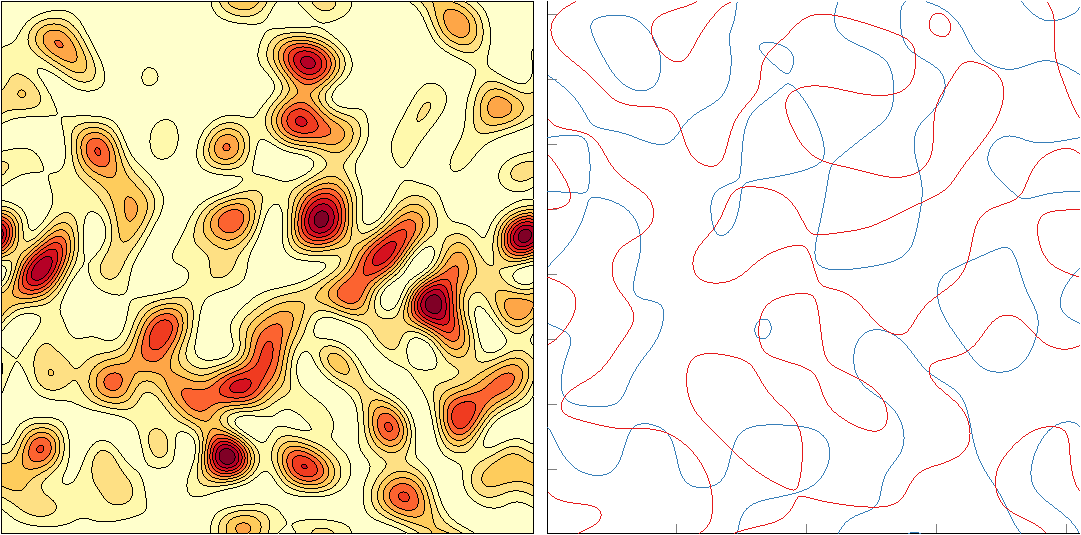
\includegraphics[keepaspectratio,width=15cm]{speckle/figures/introfig.pdf}
% ~/getvortex/specklefield.m
% make the colorbars below
\caption{Paragon speckle field, produced by the Fourier transform method.
								Right: speckle intensity.  Left: contours of the zeros of the real
								and imaginary components of the complex field, intersections of
								which are locations of optical vorticies.}
\end{figure}

When coherent waves with randomly distributed phases and amplutudes
interfere, the result exhibits seemingly random intensity fluctuations
known as \textit{speckle}.  

